\section{Local-to-Global Proof Decomposition}
\label{sec:proof-decomposition}

The formalization is best understood as proof archaeology: it takes a compact
paper proof and recovers the hidden mathematical objects one by one.  Each
object becomes necessary because a later step needs a precise support,
smoothness, or finite-sum theorem.

\subsection{The compressed paper proof}

A standard proof for compactly supported Stokes can be summarized as follows.
Choose a compact carrier \(K\) containing the support of \(\omega\).  Cover
\(K\) by finitely many coordinate neighborhoods adapted to the boundary.  Let
\((\rho_j)\) be a smooth partition of unity subordinate to that cover.  Then
write \(\omega=\sum_j \rho_j\omega\) on \(K\), apply local Stokes to each
\(\rho_j\omega\), use support to discard artificial faces, and sum the
remaining boundary terms
\cite{spivak1965calculus,guillemin1974differential,warner1983foundations,lee2013smooth,morita2001geometry}.

Every phrase in this paragraph hides a Lean obligation.

\begin{itemize}
  \item ``Cover by finitely many coordinate neighborhoods'' requires pointwise
  chart-box data, open shrink data, compactness extraction, an index type, and
  membership theorems for the selected boxes.

  \item ``Partition subordinate to the cover'' requires not merely functions
  summing to one, but topological support control strong enough to survive
  localization and coordinate transition.

  \item ``Apply local Stokes'' requires a half-space local theorem, because
  boundary charts are not ordinary Euclidean charts.

  \item ``Artificial faces vanish'' requires a theorem relating topological
  support of a zero-localized chart representative to the half-space support
  box used in the local theorem.

  \item ``Sum the remaining boundary terms'' requires a finite-sum endpoint
  reconstruction theorem, because refined boundary pieces are indexed by
  nested finite data.
\end{itemize}

The project therefore decomposes the theorem into layers.  Each layer solves a
specific mathematical problem and exposes exactly the theorem needed by the
next layer.

\subsection{Layer 1: Euclidean and half-space local Stokes}

The bottom layer is Euclidean.  The project builds on mathlib rather than
reimplementing analysis.  Local box Stokes is organized around the divergence
theorem and the coordinate form representation, following the classical
measure-theoretic and multivariable-analysis background that also underlies
formalized integration work in theorem provers
\cite{rudin1987real,evans1992measure,federer1969geometric,gouezel2022change,vandoorn2021haar}.
For boundary charts, however, the local model is the upper half-space
\[
  \HH^{n+1} = \{x : \R^{n+1} \mid 0 \le x_0\}.
\]
The formal half-space theorem has to distinguish the true lower face
\(x_0=0\) from all other faces of the coordinate box.

The key record is \code{HalfSpaceBoxInteriorStokesFields}.  It packages the
data needed to apply the Euclidean box theorem without requiring the closed
box to sit inside an ambient open subset across the boundary.  The theorem
\[
\code{halfSpaceLocalStokes_compactSupport_of_interiorFields}
\]
then says that, under the support condition killing artificial faces, the
half-space local bulk term equals the signed true boundary term.

\subsection{Layer 2: Chartwise forms and total representatives}

The next layer connects manifold forms to coordinate forms.  A chart
representative in Lean is a total function on the coordinate space.  Totality
is convenient for functions but dangerous for support statements.  The
informal support assertion
\[
  \supp(\varphi_*(\rho\omega)) \subseteq Q
\]
means that the local representative is supported in \(Q\) where the chart is
valid.  Lean must assign values outside the valid region too.  If those values
are artifacts of totalization, the ordinary support theorem is not the theorem
the proof needs.

The formal solution is the zero-localized representative
\[
\code{ManifoldForm.transitionPullbackInChartZero}.
\]
It agrees with the usual transition representative on the chart source and is
zero outside.  The project proves source, target, and overlap support
theorems for it, and then proves that localized forms constructed by the
selected smooth refinement have topological support inside their assigned
half-space boxes.

\subsection{Layer 3: Compactness to finite selected data}

Compactness enters constructively.  The first-principles theorem takes
\[
  K = \overline{\supp(\omega)}
\]
and uses compactness of \(K\).  Pointwise chart-box data is generated from the
half-space model and self charts.  From pointwise neighborhoods, the
formalization chooses open shrinks inside chart boxes, extracts a finite
selected cover, and constructs a support-controlled partition.

The phrase support-controlled is essential.  The partition is not used merely
to sum to one.  Its topological support, intersected with \(K\), must remain
inside the assigned selected open set and ultimately inside the assigned
coordinate box.  Later support theorems for localized forms depend on this
exact statement.

\subsection{Layer 4: Boundary refinement}

The boundary part requires a second finite refinement.  A selected boundary
chart may contain an active carrier that is too large for a single half-space
box.  The formal route refines each boundary active carrier into finitely many
half-space boxes and constructs smooth subpartition coefficients.  The
resulting local pieces are indexed by a pair \((i,q)\), where \(i\) is a
boundary chart index and \(q\) is a refined boundary piece.

This is one reason the endpoint layer cannot be a one-box-per-chart theorem.
The final represented endpoint is a nested finite sum, and the formalization
must keep track of the equality between the generated refined pieces and the
selected boundary finite cover.

\subsection{Layer 5: Local Stokes data to endpoint equality}

After localization and refinement, each piece has:
\begin{itemize}
  \item a half-space box with lower normal coordinate zero;
  \item a zero-localized chart representative supported in that box;
  \item analytic regularity fields sufficient for local Stokes;
  \item a local bulk term and a local true-boundary term.
\end{itemize}
The local theorem gives equality for each piece.  Finite summation gives
equality of nested sums.  The endpoint layer identifies those nested sums with
the generated represented bulk and boundary endpoints.

This decomposition explains the final theorem's shape.  Its proof is short
because each hidden mathematical step has already been turned into a named
constructor or theorem.  The short top-level proof is the result of
compression, not evidence that the theorem is a thin statement.

\begin{figure}[t]
  \centering
  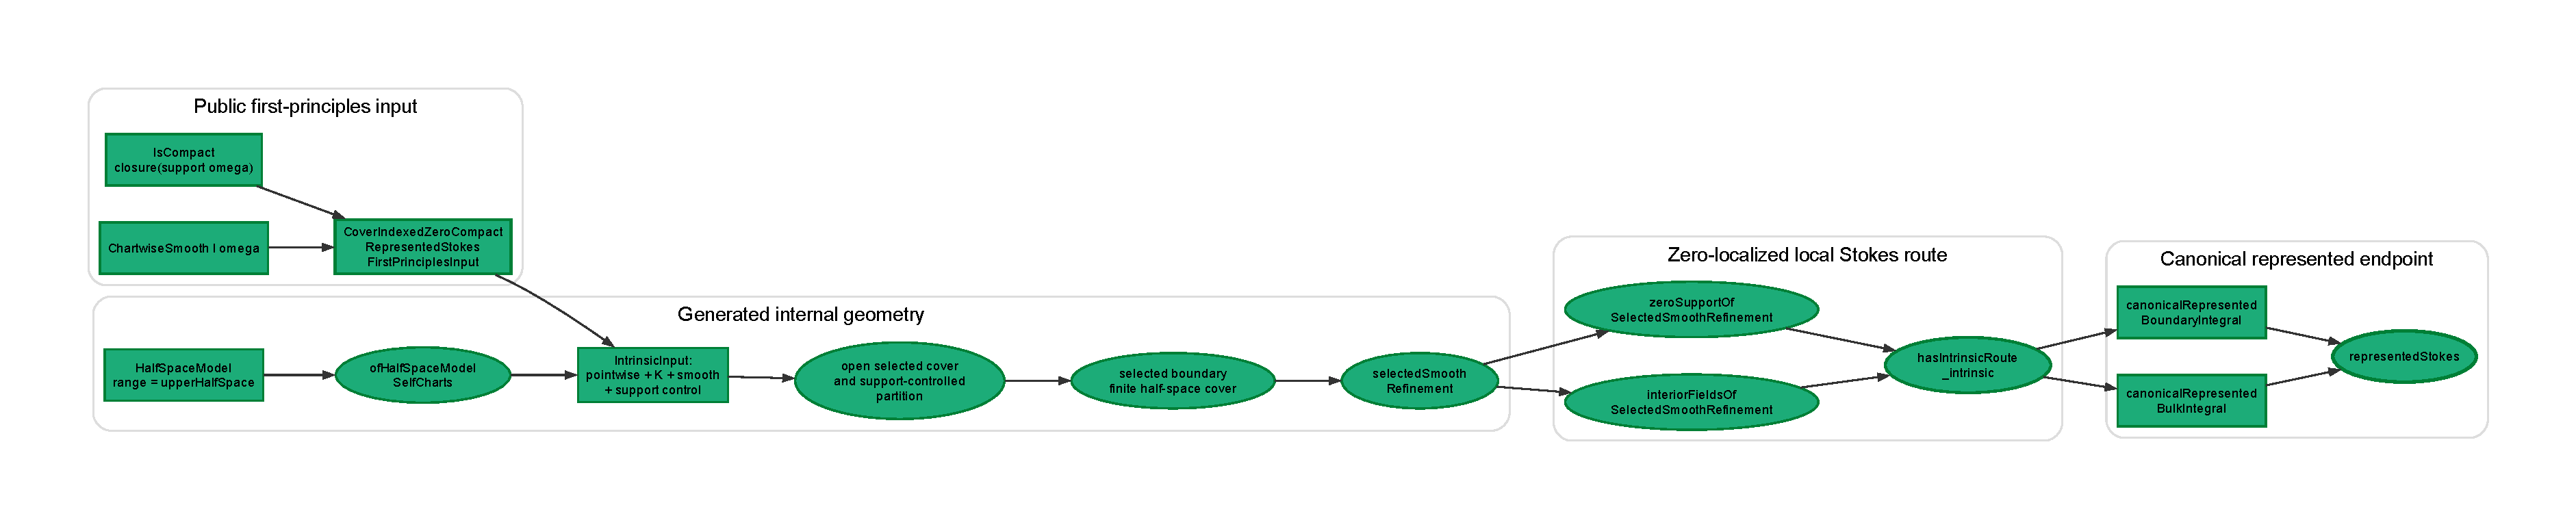
\includegraphics[width=0.94\textwidth]{figures/stokes-first-principles-graph.pdf}
  \caption{The first-principles route.  The public hypotheses generate the
  compact carrier, selected cover, support-controlled partition, smooth
  refinement, zero-localized support, local fields, and represented endpoints.
  In this and subsequent dependency figures, light-green rectangular nodes
  denote definitions or constructed data, while dark-green oval nodes denote
  theorem-level statements or derived equalities.}
  \label{fig:first-principles-route}
\end{figure}

\subsection{A useful invariant}

A recurring invariant in the development is the following:
\begin{quote}
Every local summand must carry enough support information to kill the faces
that are not part of the manifold boundary.
\end{quote}
Many intermediate certificate fields existed because this invariant had not
yet been derived from earlier data.  The final first-principles route proves
the invariant from compact support, selected open support control, and
zero-localized chart representatives.  This is the mathematical reason the
public API can be small.
